\documentclass[14pt, a4paper]{article}
\usepackage{epsfig}
\usepackage{subfigure}
%\usepackage{amscd}
\usepackage{amssymb}
\usepackage{amsbsy}
\usepackage{amsthm}
%\usepackage[dvips]{graphicx}
\usepackage{natbib}
\bibliographystyle{chicago}
\usepackage{vmargin}
% left top textwidth textheight headheight
% headsep footheight footskip
\setmargins{3.0cm}{2.5cm}{15.5 cm}{22cm}{0.5cm}{0cm}{1cm}{1cm}
\renewcommand{\baselinestretch}{1.5}
\pagenumbering{arabic}
\theoremstyle{plain}
\newtheorem{theorem}{Theorem}[section]
\newtheorem{corollary}[theorem]{Corollary}
\newtheorem{ill}[theorem]{Example}
\newtheorem{lemma}[theorem]{Lemma}
\newtheorem{proposition}[theorem]{Proposition}
\newtheorem{conjecture}[theorem]{Conjecture}
\newtheorem{axiom}{Axiom}
\theoremstyle{definition}
\newtheorem{definition}{Definition}[section]
\newtheorem{notation}{Notation}
\theoremstyle{remark}
\newtheorem{remark}{Remark}[section]
\newtheorem{example}{Example}[section]
\renewcommand{\thenotation}{}
\renewcommand{\thetable}{\thesection.\arabic{table}}
\renewcommand{\thefigure}{\thesection.\arabic{figure}}
\title{MA4605}
\author{ } \date{ }


\begin{document}
\author{Kevin O'Brien}
\title{MA4605}

\tableofcontents \setcounter{tocdepth}{2}
%-------------------------------------------------

%\chapter{Chemometrics}
\newpage

\section{About this Module}
\subsection{Rationale And Purpose Of The Module}

The extremely rapid development of analytical techniques in biology and
chemistry has left data analysis far behind, and as a result the statistical
analysis and interpretation of the data has become a major bottleneck in the
pipeline from measurement to information. \\ \noindent (Quote from ``Chemometrics with \texttt{R}", R. Wehrens,  Springer Use\texttt{R}! Series).

\begin{itemize}
\item To give students a clear understanding of the importance of statistical methods in their work.
\item To introduce students to the most widely used statistical techniques in the chemical process industries.
\item To develop skills in the use of these techniques through actual case studies using statistical software packages
\end{itemize}
\subsection{Syllabus}

%-------------------------------------------------



\begin{itemize}
\item Hypothesis testing - type I  and type II error, one and two-tailed tests, oc curves.
\item Statistical process control - various charts, mean/range, individuals/moving range, cusum charts.
\item Capability studies - capability indices.
\item Correlation and Regression - method of least squares, multiple regression, linear and non-linear models, regression analysis, analysis of residuals.
\item Importance of plotting data.
\item Design of experiments and analysis of variance - one and two way ANOVA, interaction, factorial designs, responses and factors, Plackett-Burman design, response surface methodology.
\end{itemize}
\newpage

\subsection{Recommended Text}
\begin{itemize} \item[1] Statistical Analysis Methods for Chemists (Author : William P Gardiner)
\item[2] simpleR - Using \texttt{R} for Introductory Statistics (Author : John Verzani)
\item[3] An Introduction to \texttt{R} (Authors: The R Project)
\end{itemize}

\newpage

%-------------------------------------------------
\section{Introduction to \texttt{R}}

\subsection{The \texttt{R} Project for Statistical Computing}

\texttt{R} is a language and environment for statistical computing and graphics. \texttt{R}provides a wide variety of statistical and graphical techniques, and is highly extensible. Among its tools
one can find implemented
\begin{itemize}
\item linear and nonlinear modelling,
\item classical statistical tests,
\item time-series analysis,
\item classification,
\item clustering,
\item ...and many more.
\end{itemize}
One of R's strengths is the ease with which well-designed publication quality plots can be produced.
including mathematical symbols and formulae where needed.
\begin{itemize} \item
\texttt{R} is a computing software for statistical analysis \item The package is available for all popular operating systems: Windows, Mac or Linux.
\item It is free!
\item Everyone (knowledgeable enough) can contribute to the software by
writing a package.
\item Packages are available for download through a convenient facility
\item It is fairly well documented and the documentation is available either
from the program help menu or from the web-site.
\item It is the top choice of statistical software among academic statisticians
but also very popular in industry specially among biostatisticians and
medical researchers (mostly due to the huge package called
Bioconductor that is built on the top of \texttt{R}).
\item It is a powerful tool not only for doing statistics but also all kind of
scientific programming.
\end{itemize}


\texttt{R} is an integrated suite of software facilities for data manipulation, calculation and graphical display. It
includes
\begin{itemize}
\item an effective data handling and storage facility,
\item a suite of operators for calculations on arrays, in particular matrices,
\item a large, coherent. integrated collection of intermediate tools for data analysis,
graphical facilities for data analysis and display either on-screen or on hard-copy, and
\item a well-developed, simple and effective programming language which includes conditionals, loops,
user-defined recursive functions and input and output facilities.
\end{itemize}

\subsection{Downloading and Installing \texttt{R}}

\begin{itemize}
\item \texttt{R} can be downloaded from the CRAN website: http://cran.r-project.org/
\item You may choose versions for windows, mac and linux.
\item As per the instructions on the respective pages, you require the ``base" distribution.
\item Now you can download the installer for latest version of \texttt{R} , version 2.17.
\item Select the default settings. Once you finish, the \texttt{R} icon should appear on your desktop.
\item Clicking on this icon will start up the program.
\end{itemize}

\subsection{Statistical Tables using \texttt{R}}
The following is a fragment of the tables of the values of $F(x)$ for the standard normal (`Z') cumulative distribution function from page 254 of the main textbook.
 % Reproduction of Tables

\begin{center}
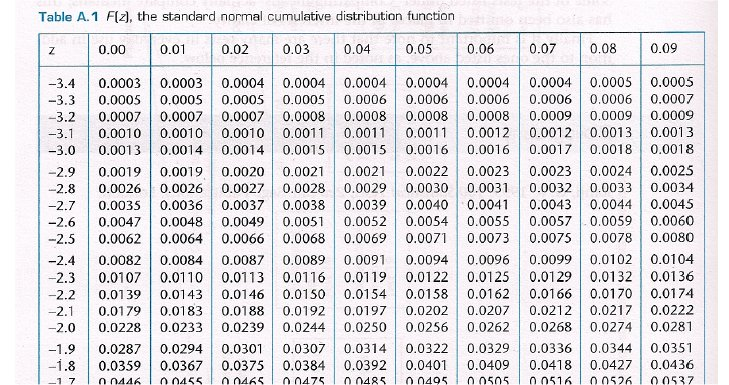
\includegraphics[scale=0.6]{Image6}
\end{center}
\newpage
\begin{center}
\line(1,0){250}
\end{center}

\begin{verbatim}
# Segment 1A-1
# Preceding line with the symbol �#� makes it a comment in R
# The following line produce a single value of the standard normal cumulative
# function. It is the value corresponding to the first value in the table

pnorm(-3.4)

#[1] 0.0003369293
#Then the first row of the table

z=seq(-3.4,-3.31,by=0.01)
pnorm(z)

# [1] 0.0003369293 0.0003494631 0.0003624291 0.0003758409 0.0003897124
# [6] 0.0004040578 0.0004188919 0.0004342299 0.0004500872 0.0004664799
# And all values from the table

z=seq(-3.4,3.4,by=0.01)
pnorm(z)

#  [1] 0.0003369293 0.0003494631 0.0003624291 0.0003758409 0.0003897124
#  [6] 0.0004040578 0.0004188919 0.0004342299 0.0004500872 0.0004664799
# [11] 0.0004834241 0.0005009369 0.0005190354 0.0005377374 0.0005570611
# [16] 0.0005770250 0.0005976485 0.0006189511 0.0006409530 0.0006636749
# [21] 0.0006871379 0.0007113640 0.0007363753 0.0007621947 0.0007888457
# [26] 0.0008163523 0.0008447392 0.0008740315 0.0009042552 0.0009354367
# [31] 0.0009676032 0.0010007825 0.0010350030 0.0010702939 0.0011066850

\end{verbatim}
\begin{center}
\line(1,0){250}
\end{center}
\newpage
There is more than meets the eye in the table. It is not only the table values that can be explored for the
standard normal distribution using \texttt{R}. Recall that the normal
distribution is defined by the density function:
\[
f(z) = \frac{1}{\sqrt(2 \pi)}e^{-Z^2/2}.
\]

The density represents distribution of probability for a random variable associated with it.
The area under the density represents the probability so the that the total area under it is equal to one.
The area accumulated up to certain value $z_o$ represents probability that a corresponding random variable takes
value smaller than z and this probability defines the cumulative distribution function $F(z)$ which is tabularized.


All this can be seen in \texttt{R}. The following code explores various aspects of the standard normal distribution:
\begin{center}
\line(1,0){250}
\end{center}
\begin{verbatim}

#Plotting the density function of the standard normal variable
z=seq(-3,3,by=0.01)
plot(z,dnorm(z),type='l',col="red",lwd=4)

#Plotting the cumulative distribution function (that one from the table)
plot(z,pnorm(z),type='l',col="red",lwd=4)

\end{verbatim}
\begin{center}
\line(1,0){250}
\end{center}
\newpage
The \texttt{R} code results in the following plots.
\begin{itemize}
\item The probability density function.
\item The cumulative density function.
\end{itemize}
\begin{center}
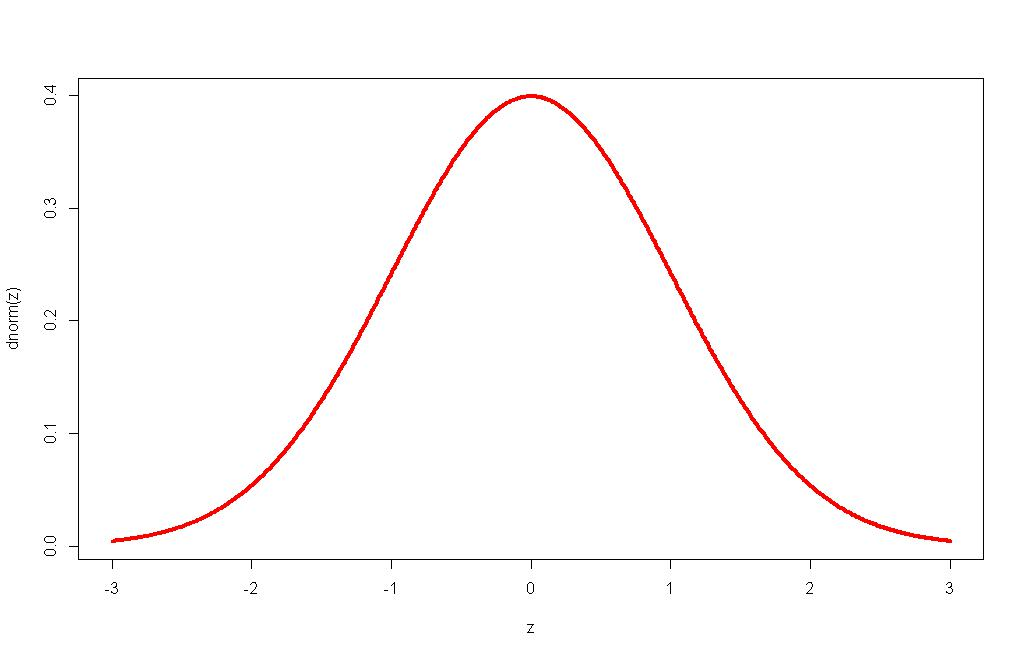
\includegraphics[scale=0.3]{Image7a}
\end{center}
\begin{center}
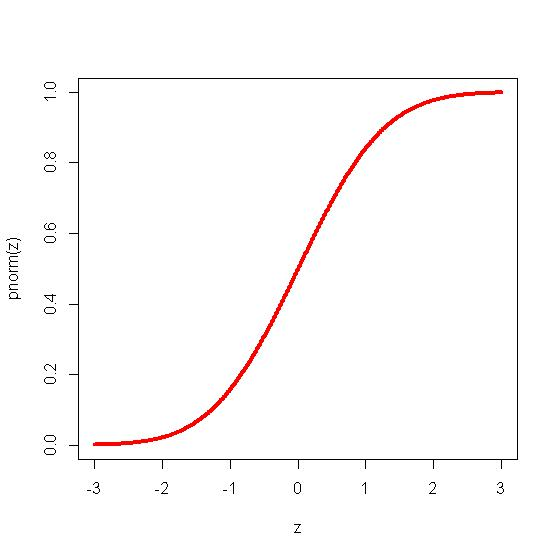
\includegraphics[scale=0.5]{Image7b}
\end{center}
\newpage
\subsection{Data Analysis with \texttt{R}}

Data from Table 1.1 of the textbook

Table 1.1 Random and systematic errors

\begin{tabular}{|c|ccccc|l|}
  \hline
  % after \\: \hline or \cline{col1-col2} \cline{col3-col4} ...
Student & Results  & (ml) &  &  &  &Comment \\ \hline
A & 10.08 & 10.11 &10.09 &10.10&10.12 & Precise, unbiased\\ \hline
B & 9.88 &10.14& 10.02 &9.80& 10.21& Imprecise unbiased\\ \hline
C & 10.19 &9.79& 9.69 &10.05& 9.78 & Imprecise, biased\\ \hline
D & 10.04 &9.98 &10.02 &9.97 &10.04 & Precise, unbiased \\
  \hline
\end{tabular}
\bigskip

This is also given in the text file Table$1-1$.txt, the contents of which is given below:
\begin{center}
\line(1,0){250}
\end{center}
\begin{verbatim}
A 10.08 10.11 10.09 10.10
B 9.88 10.14 10.02 9.80
C 10.19 9.79 9.69 10.05
D 10.04 9.98 10.02 9.97
\end{verbatim}
\begin{center}
\line(1,0){250}
\end{center}

Reading data from a file to \texttt{R}:
\begin{center}
\line(1,0){250}
\end{center}
\begin{verbatim}
#Reading the data from
Titra=read.table("Table1-1.txt", row.names = 1)
Titra
# V2 V3 V4 V5
#A 10.08 10.11 10.09 10.10
#B 9.88 10.14 10.02 9.80
#C 10.19 9.79 9.69 10.05
#D 10.04 9.98 10.02 9.97
#Listing the first row
Titra[1,]
#and the fourth column
Titra[,4]
\end{verbatim}
\begin{center}
\line(1,0){250}
\end{center}

\textbf{Means and standard deviations}\\

Find the mean and standard deviation of A's results.

\begin{center}
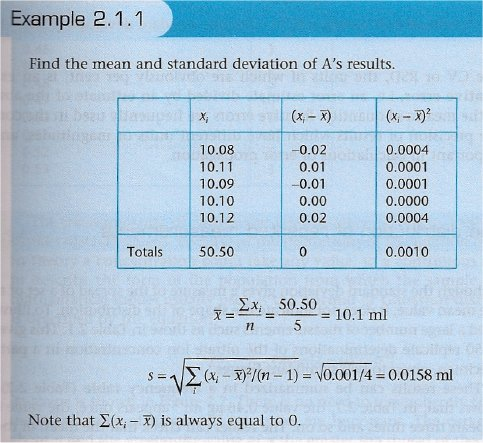
\includegraphics[scale=0.6]{Image8}
\end{center}


\textbf{Means and standard deviations much faster and better}
\begin{center}
\line(1,0){250}
\end{center}
\begin{verbatim}
#Comuting means
rowMeans(Titra)
# A B C D
#10.0950 9.9600 9.9300 10.0025
#and standard deviation
apply(Titra,1,sd)
# A B C D
#0.01290994 0.15055453 0.23036203 0.03304038
\end{verbatim}
\begin{center}
\line(1,0){250}
\end{center}
\newpage
\textbf{Nitrate ion concentration from Table 2.1}\\
Table 2.1 Results of 50 determinations of nitrate ion concentration, in $\mu$g $ml^{-1}$ (Also in the file Table $2-1$.txt.) \\
\begin{tabular}{|c|c|c|c|c|c|c|c|c|c|}
  \hline
0.51 &0.51 &0.51 &0.50 &0.51 &0.49 &0.52 &0.53 &0.50 &0.47\\
0.51 &0.52 &0.53 &0.48 &0.49 &0.50 &0.52 &0.49 &0.49 &0.50\\
0.49 &0.48 &0.46 &0.49 &0.49 &0.48 &0.49 &0.49 &0.51 &0.47\\
0.51 &0.51 &0.51 &0.48 &0.50 &0.47 &0.50 &0.51 &0.49 &0.48\\
0.51 &0.50 &0.50 &0.53 &0.52 &0.51 &0.50 &0.50 &0.51 &0.51\\
  \hline
\end{tabular}\\ \bigskip

\begin{center}
\line(1,0){250}
\end{center}
\begin{verbatim}
0.51 0.51 0.51 0.50 0.51 0.49 0.52 0.53 0.50 0.47
0.51 0.52 0.53 0.48 0.49 0.50 0.52 0.49 0.49 0.50
0.49 0.48 0.46 0.49 0.49 0.48 0.49 0.49 0.51 0.47
0.51 0.51 0.51 0.48 0.50 0.47 0.50 0.51 0.49 0.48
0.51 0.50 0.50 0.53 0.52 0.51 0.50 0.50 0.51 0.51
\end{verbatim}
\begin{center}
\line(1,0){250}
\end{center}
Compute the mean concentration, and the standard deviation:
\begin{center}
\line(1,0){250}
\end{center}
\begin{verbatim}
#Getting data in a vector
x=scan('Table2_1.txt')
mean(x)
#[1] 0.4998
sd(x)
#[1] 0.01647385
\end{verbatim}
\begin{center}
\line(1,0){250}
\end{center}
\newpage

\subsection{Bootstrap Methods}
If we would repeat our experiment of collecting 50 samples of nitrate concentrations many times we would see the range of error. But it would be a waste of resources and not a viable method.\\
Instead we re-sample `new' data from our data and use so obtained new samples for assessment of the error.
The following \texttt{R} code does the job.
\begin{center}
\line(1,0){250}
\end{center}
\begin{verbatim}
#Getting data in a vector
m=mean(x)
bootstrap=vector('numeric',500)
for(i in 1:500)
 {
 bootstrap[i]=mean(sample(x,replace=T))-mean(x)
 }
#The distribution of estimation error
hist(bootstrap)
\end{verbatim}
\begin{center}
\line(1,0){250}
\end{center}
The conclusion of this procedure is that the nitrate concentration is $4999 \pm 0.005$. We are specifically interested in how \texttt{R} was easily able to implement a solution for this.
\newpage
\section{Introduction - systematic vs. random errors}


\subsection{Quantitative nature of analytical chemistry}
Modern analytical chemistry is overwhelmingly a quantitative science.
A quantitative answer is much more valuable than a qualitative one.
It may be useful for an analyst to claim to have detected some boron in a
distilled water sample, but it is much more useful to be able to say how
much boron is present.

Often it is only a quantitative result that has any value at all.For
example, almost all samples of (human) blood serum contain albumin;
the only question is, how much ? Even where a qualitative answer is required, quantitative methods are
used to obtain it.

Quantitative approaches might be used to compare two soil samples. For example, they might be subjected to a particle
size analysis, in which the proportions of the soil particles falling within a number say 10, of particle-size ranges are determined. Each sample would then be characterized by these 10 pieces of data, which could
then be used to provide a quantitative assessment of their similarity.

\subsection{Errors in quantitative analysis}
Since quantitative studies play a dominant role in any analytical laboratory, it must be accepted that the errors that occur in such studies are of supreme importance. No quantitative results are of any value unless they are accompanied by some estimate of the errors inherent in them!
\newpage
\noindent \textbf{Example 1 - detecting a new analytical reagent}\\
\begin{itemize} \item A chemist synthesizes an analytical reagent that is believed to be entirely new.
\item The compound is studied using a spectrometric method and gives a
value of 104.
\item The chemist finds that no compound previously discovered has yielded
a value of more than 100.
\item Has the chemist really discovered a new compound?
\item The answer lies in the degree of reliance to experimental value of 104.
\item If the result is correct to within 2 (arbitrary) units, i.e. the true value
probably lies in the range $102\pm 2$, then a new material has probably
been discovered.
\item If, however, investigations show that the error may amount to 10 units
i.e. $104 \pm 10$, then it is quite likely that the true value is actually less than
100, in which case a new discovery is tar from certain.
\item A knowledge of the experimental errors is crucial!!
\end{itemize}

\newpage
\textbf{Example 2 - replicates in a titrimetric experiment}\\
\begin{itemize}
\item Analysts commonly perform several replicate determinations in the
course of a single experiment.
\item An analyst performs a titrimetric experiment four times and obtains
values of 24.69,24.73,24.77 and 25.39 ml.
\item All four values are different, because of the variations inherent in the
measurements
\item The fourth value (25.39 ml) is substantially different from the other three.
\item Can it be safely rejected, so that (for example) the mean titre is reported
as 24.73 ml, the average of the other three readings?
\end{itemize}

\subsection{Systematic and random errors}
Experimental scientists make a fundamental distinction between \textbf{\emph{random}}, and
 \textbf{\emph{systematic}} errors. To distinguish between random and systematic errors let
us consider a real experiment.\\

\noindent Four students (A-D) each perform an analysis in which exactly 10.00 $ml$
of exactly 0.1 M sodium hydroxide is titrated with exactly 0.1 NI
hydrochloric acid.
Each student performs five replicate titrations, with the results shown in
Table 1.1.
\newpage
\begin{tabular}{|c|ccccc|l|}
  \hline
  % after \\: \hline or \cline{col1-col2} \cline{col3-col4} ...
Student & Results  & (ml) &  &  &  &Comment \\ \hline
A & 10.08 & 10.11 &10.09 &10.10&10.12 & Precise, biased\\ \hline
B & 9.88 &10.14& 10.02 &9.80& 10.21& Imprecise unbiased\\ \hline
C & 10.19 &9.79& 9.69 &10.05& 9.78 & Imprecise, biased\\ \hline
D & 10.04 &9.98 &10.02 &9.97 &10.04 & Precise, unbiased \\
  \hline
\end{tabular}
\bigskip

\textbf{Graphical illustration}


The results of experiment represented by dot-plots. (The true value is 10.00).

\begin{center}
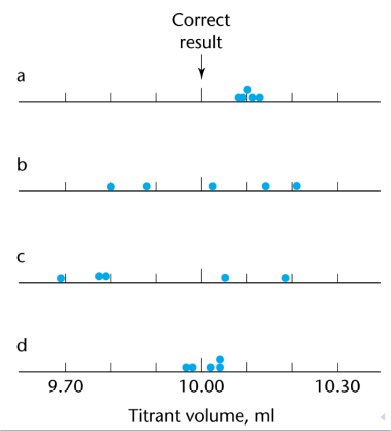
\includegraphics[scale=0.6]{Image10}
\end{center}

Recall the average for each student $ 10.0950, 9.9600, 9.9300, 10.0025 $ respectively.
\newpage

\textbf{Systematic error and bias}\\
Systematic error is a deviation of all measurements in one direction from the true value. It is well represented by the difference between the average value of the determined values and the true value
of the measured quantity. This difference is called the bias of measurements.

\textbf{Random error and precision}\\
Random error is a deviation of a measurement from the average of measured values.
It is well represented by the standard deviation of measurements.
This value is often called precision of measurements.

\textbf{Combined error vs. accuracy}\\
Accuracy is in inverse relation to the total deviation of a single measurement from the true value.



%Old Chemo 1B Finishes here
%-------------------------------------------------------%
%Old Chemo 2A Finishes here
\newpage
\section{Statistics of Repeated Measures}
\subsection{Titration experiment

Recall the titration experiment from the last class. 4 Students performing the same experiment five times, hence each yield 5 results.(Table 1.1 random and systematic errors).
\begin{tabular}{|c|ccccc|l|}
  \hline
  % after \\: \hline or \cline{col1-col2} \cline{col3-col4} ...
Student & Results  & (ml) &  &  &  &Comment \\ \hline
A & 10.08 & 10.11 &10.09 &10.10&10.12 & Precise, biased\\ \hline
B & 9.88 &10.14& 10.02 &9.80& 10.21& Imprecise unbiased\\ \hline
C & 10.19 &9.79& 9.69 &10.05& 9.78 & Imprecise, biased\\ \hline
D & 10.04 &9.98 &10.02 &9.97 &10.04 & Precise, unbiased \\
  \hline
\end{tabular}\\





Two criteria were used to compare these results, the average value (technically know
as a measure of location and the degree of spread (or dispersion). The average value
used was the arithmetic mean (usually abbreviated to \emph{the mean}), which is the sum
of all the measurements divided by the number of measurements.


The mean,$\bar{X}$, of $n$ measurements is given by \[ \bar{X}  = {\sum{x} \over n} \]

In Chapter 1 the spread was measured by the difference between the highest and
lowest values (i.e. the range). A more useful measure, which utilizes all the values, is the sample
standard deviation, $s$, which is defined as follows:

The standard deviation, $s$, of $n$ measurements is given by
\[s=  \sqrt{ {\sum(x-\bar{X})^2 \over n-1} }  (2.2) \]

\end{document}

INSERT HERE

\subsection{Means and standard deviations using \texttt{R}}
\begin{verbatim}
#Comuting means
rowMeans(Titra)
# A B C D
#10.0950 9.9600 9.9300 10.0025
#and standard deviation
apply(Titra,1,sd)
# A B C D
#0.01290994 0.15055453 0.23036203 0.03304038
\end{verbatim}

\subsection{Bias and precision using mean and standard deviation}

Classify bias and precision using means and standard deviation
of measurements.

\subsection{Measures of Dispersion}
Recall:
\begin{itemize}
\item standard deviation  = square root of variance
\item variance = squared standard deviation
\item coefficient of variation = relative standard deviation (in
percentage)
\end{itemize}

\subsection{The empirical distribution of repeated measurements}
1) frequency table
2) histogram and dotchart - graphical representation of the
empirical distribution


\textbf{Nitrate ion concentration from Table 2.1}\\
Table 2.1 Results of 50 determinations of nitrate ion concentration, in $\mu$g $ml^{-1}$
\begin{tabular}{|c|c|c|c|c|c|c|c|c|c|}
  \hline
0.51 &0.51 &0.51 &0.50 &0.51 &0.49 &0.52 &0.53 &0.50 &0.47\\
0.51 &0.52 &0.53 &0.48 &0.49 &0.50 &0.52 &0.49 &0.49 &0.50\\
0.49 &0.48 &0.46 &0.49 &0.49 &0.48 &0.49 &0.49 &0.51 &0.47\\
0.51 &0.51 &0.51 &0.48 &0.50 &0.47 &0.50 &0.51 &0.49 &0.48\\
0.51 &0.50 &0.50 &0.53 &0.52 &0.51 &0.50 &0.50 &0.51 &0.51\\
  \hline
\end{tabular}

Also in file $Table2_1.txt$
\begin{verbatim}
0.51 0.51 0.51 0.50 0.51 0.49 0.52 0.53 0.50 0.47
0.51 0.52 0.53 0.48 0.49 0.50 0.52 0.49 0.49 0.50
0.49 0.48 0.46 0.49 0.49 0.48 0.49 0.49 0.51 0.47
0.51 0.51 0.51 0.48 0.50 0,47 0.50 0.51 0.49 0.48
0.51 0.50 0.50 0.53 0.52 0.51 0.50 0.50 0.51 0.51
\end{verbatim}
The mean concentration

\noindent \textbf{Reading data}\\
\begin{verbatim}
#Getting data in a vector
x=scan("Table2_l.txt")
mean(x)
#[1] 0.4998
sd(x)
#[1] 0.01647385
\end{verbatim}

\textbf{Dotchart and histogram in R}\\
\begin{verbatim}
#Dotchart
dotchart(x)
#Histogram and frequency table
Histogr=hist(x)
Histogr
\end{verbatim}

\subsection{The Normal Distribution - Theoretical distribution of repeated measurements}

It is not only the table values that can be explored for the
standard normal distribution using \texttt{R}. Recall that the normal
distribution is defined by the density

\[
f(z) = \frac{1}{\sqrt(2 \pi)}e^{-Z^2/2}.
\]

The density represents distribution of probability for a random variable associated with it.
The area under the density represents the probability so the that the total area under it is equal to one.
The area accumulated up to certain value $z$ represents probability that a corresponding random variable takes
value smaller than $z$ and this probability defines the cumulative distribution function $F(z)$ which is tabularized.


\textbf{Normal distribution in R}\\
The following code explores various aspects of the standard normal distribution

\begin{verbatim}
#Plotting the density function of the standard normal variable
z=seq(-3,3,by=0.01)
plot(z,dnorm(z),type="l",col="red",lwd=4)

#Plotting the cumulative distribution function (that one from the table)
plot(z,pnorm(z),type="l",col="red",lwd=4)

#And plotting them one at the top of the other
par(mfrow=c(2, 1))
plot(z,dnorm(z),type="l",col="red",lwd=4)
plot(z,pnorm(z),type="l",col="red",lwd=4)

#Side by side
par(mfrow=c(1, 2))
plot(z,dnorm(z),type="l",col="red",lwd=4)
plot(z,pnorm(z),type="l",col="red",lwd=4)
\end{verbatim}

\subsection{Empirical vs Theoretical}
The theoretical one can be compared with empirical by taking $\mu$ equal to the sample mean $\bar{X}$ and $\sigma$  equal to sample standard deviation $s$.
The following code compares empirical percentages with theoretical.
\begin{verbatim}
quantile(x,c(0.16,0.84))
qnorm(c(0.16,0.84),mean(x),sd(x))
\end{verbatim}


\textbf{Example 2.2.1}If repeated values of a titration are normally distributed with mean 10.15 ml
and standard deviation 0.02 ml, find the proportion of measurements which
lie between 10.12 ml and 10.20 ml.

Standardizing the first value gives \[z = (10.12 - 10.15)/0.02 = -1.5.\]
From Table A.1, $F(-1.5) = 0.0668$.

Standardizing the second value gives \[ z = (10.20 - 10.15)/0.02 = 2.5.\]
From Table A.1, $F(2.5) = 0.9938$.

Thus the proportion of values between x = 10.12 to 10.20 (which corresponds
to z =-1.5 to 2.5) is $0.9938 - 0.0668 = 0.927$.

No standardization needed in \texttt{R}
\begin{verbatim}
pnorm(c(10.12,10.20),10.15,0.02)
\end{verbatim}

Not everything is normal, unfortunately - lognormal distribution
\begin{verbatim}
Concentr=scan("Figure2-5.txt")
hist(Concentr)
hist(Concentr,nclass=30)
\end{verbatim}

\textbf{Distribution of the sample mean}
\begin{verbatim}
MatrConc=matrix(Concentr,ncol=4)
ConcM=rowMeans(MatrConc)
hist(ConcM)
MatrConc=matrix(Concentr,ncol=25)
ConcM=rowMeans(MatrConc)
hist(ConcM)
\end{verbatim}

\subsection{Two distributional effects of taking sample mean}
\begin{itemize}
\item Reduction in standard deviation (increased precision)
\item Distribution is becoming normal even if original is not.
\end{itemize}
For a sample of $n$ measurements,standard error of the mean
\[S.E.(\bar{X}) = {\sigma \over \sqrt{n}} (2.5)\]

As expected, the larger n is, the smaller the value of the s.e.m. and consequently the
smaller the spread of the sample means about $n$.
The term 'standard error of the mean' might give the impression that o'/W gives
the difference between $mu$ and $\bar{X}$. This is not so: $\sigma / \sqrt{N}$ gives a measure of the variability of $\bar{X}$, as we shall see in the next section.

Another property of the sampling distribution of the mean is that, \emph{even if the original population is not normal}, the sampling distribution of the mean tends to the normal distribution as n increases. This result is known as the \emph{\textbf{central limit theorem}}. This theorem is of great importance because many statistical tests are performed on the mean and assume that it is normally distributed.

Since in practice we can assume that distributions of repeated measurements are at least approximately normally distributed, it is reasonable to assume that the means of quite small
samples (say $n>5$) are normally distributed.


\section{Confidence Intervals}

\subsection{Large sample distribution of sample mean}
%Chemo 2009 2B

\subsection{Confidence limits of the mean for large samples}
Now that we know the form of the sampling distribution of the mean we can return to the problem of using a sample to define a range which we may reasonably assume includes the true value. (Remember that in doing this we are assuming systematic errors to be absent.) Such a range is known as a confidence interval and the extreme values of the range are called the confidence limits.

The term 'confidence' implies that we can assert with a given degree of confidence, i.e. a ' certain probability, that the confidence interval does include the true value.

The size of the confidence interval will obviously depend on how certain we want to be that it includes the true value: the greater the certainty, the greater the interval required.

Figure 2.6 shows the sampling distribution of the mean for samples of size $n$. If we assume that this distribution is normal then $95\%$  of the sample means will lie in the range given by:
\[ \mu - 1.96(\sigma/\sqrt{n}) < \mu < \mu + 1.96(\sigma/\sqrt{n}) (2.6)\]

(The exact value 1.96 has been used in this equation rather than the approximate
value, 2, quoted in Section 2.2. The reader can use Table A.1 to check that the pro-
portion of values between z= -1.96 and z = 1.96 is indeed 0.95,)

\subsection{Large Sample Confidence Intervals based on the sample mean}

In practice, however, we usually have one sample, of known mean, and we require a range for $\mu$, the true value.

Equation (2.6) can be rearranged to give this:
\[ \bar{X} - 1.96(\sigma/\sqrt{n}) < \mu < \bar{X} + 1.96(\sigma/\sqrt{n}) (2.7)\]

Equation (2.7) gives the $95\%$  confidence interval of the mean. The $95\%$  confidence
limits are $\bar{X} \pm 19.6 \sigma/\sqrt{n}$
In practice we are unlikely to know $\sigma$ exactly. However, provided that the sample is
large, $\sigma$ can be replaced by its estimate, $s$.


\subsection{Example of computations using R}
Finding confidence intervals for the mean for the nitrate ion
concentrations in Table 2.1.
\begin{verbatim}
#reading data
x=scan("Table2_1.txt")
#setting the confidence level
CL=0.95
#computing confidence interval
n=length(x)
pm=sd(x)*c(qnorm(0.025),qnorm(0.975))/sqrt(n)
CI=mean(x)+pm
\end{verbatim}

\subsection{Small-Sample Case (n < 30)}
If the data have a normal probability distribution and the sample
standard deviation s is used to estimate the population
standard deviation $s$, the interval estimate is given by:
\[ \bar{X} \pm t_{\alpha/2}s /\sqrt{n} \]
where $\alpha/2$ is the value providing an area of $\alpha/2$  in the upper tail
of a Student's $t-$distribution with n - 1 degrees of freedom.


\subsection{Confidence limits of the mean for small samples}

As the sample size gets smaller, s becomes less reliable as an estimate of $\sigma$. This can
be seen by again treating each column of the results in Table 2.2 as a sample of size
five. The standard deviations of the 10 columns are 0.009, 0.015, 0.026, 0.021
0.013, 0.019, 0.013, 0.017, 0.010 and 0.018. We see that the largest value of $s$ is
nearly three times the size of the smallest. To allow for this, equation (2.8) must be
modified.

For small samples, the confidence limits of the mean are given by
\[ \bar{X} \pm t_{n-1}s /\sqrt{n} \]


\subsection{Student t-distribution}

Values for confidence interval of $95\%$ and $99\%$
\begin{tabular}{|c|c|c|}
  \hline
  % after \\: \hline or \cline{col1-col2} \cline{col3-col4} ...
  Degrees of Freedom & $95\%$ & $95\%$ \\ \hline
  2 & 4.30 & 9.92 \\
  5 & 2.57  & 4.03 \\
  10 & 2.23 & 3.17 \\
  20 & 2.09 & 2.85 \\
  50 & 2.01 & 2.68 \\
  100 & 1.98 & 2.63 \\
  \hline
\end{tabular}


The subscript (n - 1) indicates that r depends on this quantity, which is known as the
number of degrees of freedom, d.f. (usually given the symbol $\nu$). The term ``degrees
of freedom" refers to the number of independent deviations ($x-bar{x}$) which are used in
calculating the sample standard deviation$s$.

In this case the number is $(n- 1)$, because when $(n - 1)$ deviations are
known the last can be deduced since $\sum x-bar{x} = 0$.

The value of $t$ also depends on the degree of confidence required. Some values of $t$ are given in Table 2.3.
A more complete version of this table is given in Table A.Z in Appendix 2 of the recommended text.

For large $n$, the values of $t_{n-1}$ for confidence intervals of $95\%$ and $99\%$ respectively
are very close to the values 1.96 and 2.58 used in Example 2.6.1.




\subsection{Why "Student"?}

William S. Gosset was a statistician , employed by the Guinness brewing
company which had stipulated that he not publish under his own name.
He therefore wrote under the pen name "Student." His main contribution was published in 1908.

\subsection{Example of computations using R}
Finding confidence intervals for the mean for the nitrate ion
concentrations in Example 2.7.1.
\begin{verbatim}
#Typing data in
x=c(lO2,97,99,98,101,106)
mean(x)
sd(x)
n;length(x)
#setting the confidence level
CL=O.95
#computing confidence interval
pm=sd(x)*c(qt(0.025,n-l),qt(O.975,n-l))/sqrt(n)
CI=mean(x)+pm
\end{verbatim}

% Old Chemo 2B finishes here
\end{document}
%---------------------------------------%
% Old Chemo 3A starts here

\section{Propagation of random errors}

\subsection{Linear combination}
Propagation of the error in the linear combination of independent measurements

\noindent \textbf{Linear combinations (2.11.1)}

In this case the final value, y, is calculated from a linear combination of measured
quantities $a$, $b$, $c$, etc., by:
\[k +k_aa+k_bb+k_cc\ldots (2.10)\]
where $k$, $k_a$, $k_b$, $k_c$ etc., are constants. Variance (defined as the square of the standard
deviation) has the important property that the variance of a sum or difference of
independent quantities is equal to the sum of their variances. It can be shown that if
$\sigma_a$, $\sigma_b$,$\sigma_c$, etc., are the standard deviations of $a$, $b$, $c$, etc., then the standard deviation
of y, $\sigma_y$,, is given by:
\[ \sigma_y = \sqrt{(k_a\sigma_a)^2 + (k_b\sigma_b)^2 + (k_c\sigma_c)^2 + \ldots}\]

\textbf{Illustration in R}\\
Illustration using random samples generated by R:
\begin{verbatim}
#generating data
#initial reading
x=rnorm(100,3.51,0.02)
#final reading
y=rnorm(100,15.67,0.02)
#volume used
z=y-x
mean(x)
mean(y)
mean(z)
sd(x)
sd(y)
sd(z)
sqrt(var(x)+var(y))
\end{verbatim}

\subsection{Multiplicative expressions}
The following is true only approximately. Still measurements are assumed to be independent.

\noindent \textbf{Multiplicative expressions (2.11.2)}\\
If y is calculated from an expression of the type;
\[ y = \frac{kab}{cd} (2.12)\]

(where a, b, c and d are independent measured quantities and k is a constant) then
there is a relationship between the squares of the relative standard deviations:

\[ \frac{\sigma_y}{\mu_y} = \sqrt{(\frac{\sigma_a}{\mu_a})^2 + (\frac{\sigma_b}{\mu_b})^2 + (\frac{\sigma_c}{\mu_c})^2 + \ldots} (2.13)\]

\subsection{Example}

The quantum yield of fluorescence, $\phi$, is calculated from the expression:
\[\phi = Qkclloe)\]
where the quantities involved are defined below, with an estimate of the
relative standard deviations in brackets:

$I_o$ = incident light intensity $(0.5\%)$\\
$I_f$ = fluorescence intensity $(2\%)$\\
$\epsilon$ = molar absorptivity $(1\%)$\\
$c$ = concentration $(0.2\%)$\\
$l$ = path-length $(0.2\%)$\\
$k$ is an instrument constant.\\
From equation (2.13), the relative standard deviation of o is given by:
RSD : V22 + 0.22 + 0.22 + 0.52*+-? = 2.3%

\subsection{Illustration in R}

\textbf{Illustration using random samples generated by \texttt{R}:}

\begin{verbatim}
#generating data

#incident light intensity
I0=rnorm(100,10,0.005*10)

#fluorescence intensity
If=rnorm(100,15,0.02*15)

#molar absorptivity
e=rnorm(100,5,0.01*5)

#concentration
c=rnorm(100,2,0.002*2)

#path-length
l=rnorm(100,11,0.002*11)

#Computing quantum yield of fluorescence
phi=If/(c*l*I0*e)
sd(x)/mean(phi)
\end{verbatim}

%----------------------------------- Chemometrics 4B5A
\subsection{One-sided vs. two-sided test}
% 2 - 6
We consider the null hypothesis:
$H_o : \mu = \mu_0$
where $\mu$ is unknown but true value of the mean while $\mu_0$ is a
known hypothesized value of the true mean.
We want to detect if 6= 0. Alternatively, we can consider the
null hypothesis:
$H_o : \mu \leq \mu_0$
and we want to detect if \mu > \mu_0$.
In the first case, we deal with a
two-sided test while the second case is described as a
one-sided one.

%------------------------------------------------%
%-- Pg 7

%------------------------------------------------%
%-- Pg 8
\begin{verbatim}
x=c(25.06, 25.18, 24.87, 25.51, 25.34, 25.41)
t.test(x,mu=25, alternative="greater")
\end{verbatim}

%------------------------------------------------%
%-- Pg 9 - 11
\section{F-test for comparison of variances}

We consider the null hypothesis:
$H_o : \sigma^2_1 = \sigma^2_1$

and we want to detect if $\sigma^2_1 \neq \sigma^2_1$

Alternatively, in one-sided
version the alternative is $\sigma^2_1 > \sigma^2_1$

We take the ratio
\[ F = \frac{s^2_1}{s^2_2} \]

and consider this having the so-called F-distribution (Fisher�s
distribution) with $(n_1-1)$ and $(n_2-1)$ degrees of freedom.
%------------------------------------------------%
%-- Pg 12

\begin{verbatim}
F-distribution in R
n1=6
n2=12
r=seq(0.01,10,by=0.01)
plot(r,df(r,n1-1,n2-1))
\end{verbatim}

%------------------------------------------------%
%-- Pg 13


%------------------------------------------------%
%-- Pg 14


%------------------------------------------------%
%-- Pg 15
\subsection{Example 3.6.1 in R}
\begin{verbatim}
alpha=0.05
n1=8
n2=8
s1=3.31
s2=1.51
f=s1�2/s2�2
r=seq(0.01,10,by=0.01)
plot(r,df(r,n1-1,n2-1))
points(qf(1-alpha,n1-1,n2-1),0,pch="o",col="blue")
points(f,0,pch="*",col="red")
pvalue=1-pf(f,n1-1,n2-1)
pvalue
\end{verbatim}


%------------------------------------------------%
%-- Pg 16


%------------------------------------------------%
%-- Pg 17



%------------------------------------------------%
%-- Pg 18
\begin{verbatim}
alpha=0.05
n1=5
n2=5
s1=0.31
s2=0.28
f=s1�2/s2�2
r=seq(0.01,10,by=0.01)
plot(r,df(r,n1-1,n2-1))
points(c(qf(alpha/2,n1-1,n2-1),qf(1-alpha/2,n1-1,n2-points(f,0,pch="*",col="red")
pvalue=min(pf(f,n1-1,n2-1),1-pf(f,n1-1,n2-1))
pvalue
\end{verbatim}
%------------------------------------------------%
%-- Pg 19


%------------------------------------------------%
%-- Pg 20

%------------------------------------------------%
%-- Pg 21


%------------------------------------------------%
%-- Pg 22

%------------------------------------------------%
%-- Pg 23
\subsection{Outliers in R}
The tests for outliers come in a contributed package called
�outliers�. In order to use it one has to download the package to
the computer. It can be done for the command line by using
install.package("outliers") or can by using a
convenient interface of the software.
\begin{verbatim}
x=c(0.403,0.410,0.401,0.380)
grubbs.test(x)
# Grubbs test for one outlier
#data: x
#G = 1.4316, U = 0.0892, p-value = 0.09124
#alternative hypothesis: lowest value 0.38 is an outlier
\end{verbatim}

%------------------------------------------------%
%-- Pg 24
\begin{verbatim}
dixon.test(x)
# Dixon test for outliers
#data: x
#Q = 0.7, p-value = 0.1721
#alternative hypothesis: lowest value 0.38 is an outlier
x=c(0.403,0.410,0.401,0.380,0.400,0.413,0.408)
grubbs.test(x)
dixon.test(x)
\end{verbatim}
%------------------------------------------------%
%-- Pg 25-30

\subsection{The chi-squared test for proportions}

Supposed that we have several categories of events that are
observed.
Assume that $n$ observations are made in total and there is $k$
disjoint categories to which they can be classified.
Let $O_i$ represent the observed count in the ith category.
Let $p_i$ be the proportion of the count that is expected in the ith
category, so that the expected count for this category is $E_i = np_i$ .
Consider the quantity
\[ \chi^2 = \sum^{k}_{i=1}\frac{(O_i-E_i)^2}{E_i} \]

and reject assumed proportions $p_i$ if $\chi^2$ is too large.

%----------------------------------------------%
%pg 31 - Blank
%pg 32 - Graphics
%pg 33 long example
%pg 34
Report form R
\begin{verbatim}
qchisq(0.95,3)
[1] 7.814728
1-pchisq(8.966,3)
[1] 0.02974637
\end{verbatim}
%pg 35-36 Testing for Normality

\subsection{Testing for normality of distribution}
The chi-square test could be used for testing normality by
dividing the range of data into bins and compare the count in
each bin with the corresponding probabilities based on the
normal distribution.
Unfortunately, one needs relatively large data sample size in
order to use chi-squared test ($> 50$), thus there is a need for a
small sample size procedure.

\subsection{Normaly Probability Plots}
%pg 37-39
Normal probability plots
One simple graphical way of comparing data to normal
distributions is by plotting empirical quantile vs.
corresponding normal quantile.
Recall that the p-quantile for a given (empirical) distribution
is the number below of which there is 100p% of probability
(of the data).
Consider data from Example 3.12.1
x=c(109,89,99,99,107,111,86,74,115,107,134,113,110,88,104)
The normal probability plot is obtained in R using
qqnorm(x)

%pg 40
\subsection{KS test}

%pg 41

Kolmogorov-Smirnov test in R
\begin{verbatim}
x=c(25.13,25.02,25.11,25.07,25.03,24.97,25.14,25.09)
ks.test(x,"pnorm",mean(x),sd(x))
One-sample Kolmogorov-Smirnov test
data: x
D = 0.1321, p-value = 0.995
alternative hypothesis: two-sided
\end{verbatim}


\subsection{Types of errors}
Consider the testing statistical hypothesis
$H0 : \mu = 3.0\%$
against
$H1 : \mu = 3.5\%$
Significance level $\mu$ (typically $5\%$) represents chances of rejecting $H_0$
given that it is true.
We refer to this as the probability of Type I Error.
The other error we can make is saying that we do not reject $H_0$ while in
fact $H_1$ is true. This is called Type II Error.
One minus probability of
making Type II Error is called the power of the test.

\sbsection{Calculation of the power}
We reject $H_0$ if $t = (\bar{x} - 3.0)/(0.036/\sqrt{n}) > 1.96$, where n = 4, or
equivalently if $\bar{x} > 0:036 \times (1.96/\sqrt{n})  + 3.0 = 3.035$.

If H1 is true, then $x > 3.035$ is given by chances that the normal variable that
has mean 3.05 and variance 0.036/2 exceeds 3.035 which is
\end{verbatim}
1-pnorm(3.035,3.05,0.036/2)
0.7976716
\end{verbatim}
Thus the power of this test is about 80%.

The power and sample size
In general, the power depends on the sample size. We reject H0 if
t = ( x ?? 3:0)=(0:036=pn) > 1:96, where n = 4, or equivalently if
x > 0:036 1:96=pn + 3:0.
If H1 is true, then x > 0:036 1:96=pn + 3:0 is a function of n that
can be plotted as follows
n=1:100
plot(n,1-pnorm(0.036*1.96/sqrt(n)+3.0,3.05,0.036/2),col="red")

\end{document}




%--------------------------------------%

\section{Statistical Inference} What is Statistical Inference?
\begin{itemize}\item Hyptothesis testing \item Confidence
Intervals \item Sample size estimation.\end{itemize}

\subsection{Hypothesis testing: introduction}
The objective of hypothesis testing is to access the validity of a claim against a counterclaim using sample data
\begin{itemize}\item The claim to be �proved� is the alternative hypothesis($H_1$).\item The competing claim is called the null hypothesis($H_0$).\item One begins by assuming that $H_0$ is true. \end{itemize}

If the data fails to contradict $H_0$ beyond a reasonable doubt, then $H_0$ is not rejected. However, failing to reject $H_0$ does not mean that we accept it as true. It simply means that $H_0$ cannot be ruled out as a possible explanation for the observed data. A proof by insufficient data is not a proof at all.

\begin{quote}
�The process by which we use data to answer questions about parameters
is very similar to how juries evaluate evidence about a defendant.� �from
Geoffrey Vining, Statistical Methods for Engineers, Duxbury, 1st edition,
1998.
\end{quote}
\section{Confidence Intervals}

\section{Hypothesis Testing}


Hypothesis testing is a common practice in science that involves conducting tests and experiments to see if a proposed explanation for an observed phenomenon works in practice. A hypothesis is a tentative explanation for some kind of observed phenomenon, and is an important part of the scientific method. The scientific method is a set of steps that is commonly employed by those in scientific fields to give scientific explanations for various phenomena.

Any tentative explanation can be referred to as a hypothesis if it can be submitted to hypothesis testing. There are, however, a set of guidelines for an explanation to be considered a true scientific hypothesis. The first major point is testability; a scientific hypothesis must be able to proceed to the stage of hypothesis testing to be considered a scientifically legitimate hypothesis. It is generally suggested that a hypothesis be relatively simple, though this is not always possible. Hypotheses must also be able to explain the phenomena under any set of conditions; if a hypothesis can only explain a phenomenon in one set of conditions, it is generally considered unacceptable.

Hypotheses are generally considered useful only if they are likely to improve on the current body of knowledge on a subject and pave the way for greater knowledge to be acquired in the future. Also, a hypothesis is generally not acknowledged if it defies other commonly recognized knowledge. If a hypothesis meets all of these requirements, it will typically proceed to the hypothesis testing phase.

In hypothesis testing, the testers seek to discover evidence that either validates or disproves a given hypothesis. Usually, this involves a series of experiments being conducted in many different conditions. If the hypothesis does not stand up to the tests in all conditions, something is usually wrong with the hypothesis and a new one must be formed to take the new information into account. The new hypothesis is submitted to the same hypothesis testing. If it passes and is not proven wrong, it can eventually be considered a scientific theory or law, though nothing in science can be proven to be absolutely true.

One common method of hypothesis testing is known as statistical hypothesis testing, and typically deals with large quantities of data. Experiments and tests are conducted and the data is collected. If the data collected shows that it is unlikely that the results occurred by chance, it is considered statistically significant and can be used to support a hypothesis.


\section{Degrees of Freedom}

Degree of freedom (df) is a concept most used in statistics and physics. In both cases it tends to define limits of a system and position or size of what is being analyzed, so that it can be visually represented. Definition of df in both fields is related, but not quite the same.

In physics, degree of freedom positions objects or systems, and each degree references a position in time, space or in other measurements. Df could be used synonymously with the term coordinate, and it usually means independent coordinates of the fewest number. The actual degree of freedom is based on the system being described in phase space or in all the potential types of space a system inhabits simultaneously. Every single part of phase space the system takes up can be considered a df, which helps to define the full realities of the system being considered.

From a statistical standpoint, degree of freedom defines distributions of populations or samples and is encountered when people begin to study inferential statistics: hypothesis testing and confidence intervals. As with the scientific definition, df in statistics describes shape or aspects of sample or population depending on data. Not all drawn representations of distributions have a degree of freedom measurement. The common standard normal distribution is not defined by degrees; instead, it will be the same bell-shaped curve in all instances.

A similar distribution to standard normal is student-t. The student-t is defined in part by degree of freedom in the formula n-1, where n is sample size. This means that were variables from the distribution to be picked one by one, all but the last one could be chosen freely. There is no choice but to take the very last one and no freedom to choose any other variable at that point. Therefore one variable is not free; it�s like having to pick the last tile out of a bag during a Scrabble� game where there is no choice but to choose that letter.

Different distributions like the F and the chi-square have different definitions of degree of freedom, and some even use more than one df in definition. The issue gets confusing because df definition is linked to type of test performed and isn�t the same with the various parametric (based on parameters) and non-parametric (not based on parameters) tests. Essentially, it won�t always be n-1. Goodness of fit or contingency table testing may use the chi-square distribution with different df than that which evaluates single variable hypothesis testing of the variance or standard deviation.

What is important to remember is that each time degree of freedom is used to define a distribution, it changes it. It still may have certain characteristics that are unchanging, but size and appearance vary. When people are drawing representations of distributions, particularly two of the same distributions that have a different df, they�re advised to make them look different in size to convey that df is not the same.



\section{Statistical significance}

Statistical significance is a mathematical tool used to determine whether the outcome of an experiment is the result of a relationship between specific factors or due to chance. Statistical significance is commonly used in the medical field to test drugs and vaccines and to determine causal factors of disease. Statistical significance is also used in the fields of psychology, environmental biology, and any other discipline that conducts research through experimentation.

Statistics are the mathematical calculations of numeric sets or populations that are manipulated to produce a probability of the occurrence of an event. Statistics use a numeric sample and apply that number to an entire population. For the sake of example, we might say that $80\%$ of all Americans drive a car. It would be difficult to question every American about whether or not they drive a car, so a random number of people would be questioned and then the data would be statistically analyzed and generalized to account for everyone.

In a scientific study, a hypothesis is proposed, then data is collected and analyzed. The statistical analysis of the data will produce a number that is statistically significant if it falls below $5\%$, which is called the confidence level. In other words, if the likelihood of an event is statistically significant, the researcher can be $95\%$ confident that the result did not happen by chance.

Sometimes, when the statistical significance of an experiment is very important, such as the safety of a drug meant for humans, the statistical significance must fall below $3\%$. In this case, a researcher could be $97\%$ sure that a particular drug is safe for human use. This number can be lowered or raised to accommodate the importance and desired certainty of the result being correct.

Statistical significance is used to reject or accept what is called the null hypothesis. A hypothesis is an explanation that a researcher is trying to prove. The null hypothesis holds that the factors a researcher is looking at have no effect on differences in the data. Statistical significance is usually written, for example, $t=.02, p<.05$. Here, "t" stands for the statistic test score and "p<.05" means that the probability of an event occurring by chance is less than $5\%$. These numbers would cause the null hypothesis to be rejected, therefore affirming that the alternative hypothesis is true.

Here is an example of a psychological hypothesis using statistical significance: It is hypothesized that baby girls smile more than baby boys. In order to test this hypothesis, a researcher would observe a certain number of baby girls and boys and count how many times they smile. At the end of the observation, the numbers of smiles would be statistically analyzed.

Every experiment comes with a certain degree of error. It is possible that on the day of observation all the boys were abnormally grumpy. The statistical significance found by the analysis of the data would rule out this possibility by 95\% if t=.03. In this case, the null hypothesis that baby girls do not smile more than baby boys would be rejected, and with 95\% certainty, the researcher could say that girls smile more than boys.



\section{Fisher's exact test}

Fisher's exact test is a statistical significance test used for small sample sizes. It is one of a number of tests used to analyze contingency tables, which display the interaction of two or more variables. Fisher's exact test was invented by English scientist Ronald Fisher, and it is called exact because it calculates statistical significance exactly, rather than by using an approximation.

To understand how Fisher's exact test works, it is essential to understand what a contingency table is and how it is used. In the simplest example, there are only two variables to be compared in a contingency table. Usually, these are categorical variables. As an example, imagine you are conducting a study on whether gender correlates with owning pets. There are two categorical variables in this study: gender, either male or female, and pet ownership.

A contingency table is set up with one variable on the top, and the other on the left side, so that there is a box for each combination of variables. Totals are given on the bottom and at the far right. Here is what a contingency table would look like for the example study, assuming a survey of 24 individuals:
\begin{verbatim}
 Pet Owner Not a Pet Owner Total
Male 1 9 10
Female 11 3 14
Total 12 12 24
\end{verbatim}
Fisher's exact test calculates deviance from the null hypothesis, which holds that there is no bias in the data, or that the two categorical variables have no correlation with each other. In the case of the present example, the null hypothesis is that men and women are equally likely to own pets. Fisher's exact test was designed for contingency tables with a small sample size, or large discrepancies between cell numbers, like the one shown above. For contingency tables with a large sample size and well-balanced numbers in each cell of the table, Fisher's exact test is not accurate, and the chi-square test is preferred.

In analyzing the data in the table above, Fisher's exact test serves to determine the probability that pet-ownership is unevenly distributed among men and women in the sample. We know that ten of the 24 people surveyed own pets, and that 12 of the 24 are female. The probability that ten people chosen at random from the sample will consist of nine women and one man will suggest the statistical significance of the distribution of pet owners in the sample.

Probability is denoted by the letter p. Fisher's exact test determines the p-value for the above data by multiplying the factorials of each marginal total -- in the table above, 10, 14, 12, and 12 -- and dividing the result by the product of the factorials of each cell number and of the grand total. A factorial is the product of all positive integers less than or equal to a given number. $10!$, pronounced "ten factorial," is therefore equal to $10\times 9\times8 \times \ldots\times 3 \times 2 \times 1$, or 3,628,800.

For the table above, then, $p= (10!)(14!)(12!)(12!)/(1!)(9!)(11!)(3!)(24!)$. Using a calculator, one can determine that the probability of getting the numbers in the table above is under $2\%$, well below chance, if the null hypothesis is true. Therefore, it is very unlikely that there is no contingency, or significant relationship, between gender and pet-ownership in the study sample.


Continuous data protection is a type of backup system that allows for information on a computer system to be constantly backed up on a different server, possibly even at a different physical location. Many consider this to be one of the safest forms of backup protection. While some systems back up the information stored on the main computer every day or even every few days, continuous data protection ensures that not even a day's work is lost in the event of a catastrophic computer failure.

In most cases, continuous data protection works by saving an exact copy of a file a user is working with to a different location. Each time the user changes the file, a new file is saved remotely, usually overwriting the previous file saved under that same name. Thus, it is not real-time backup in that each keystroke or move of the mouse is recorded and saved. That may be a very important distinction for those who are expecting to recover lost work because of things like power failures, where a computer will shut down unexpectedly. Real-time backup products are also available, for those who want them.

Computer users can utilize continuous data backup in a number of different ways. Software products currently on the market allow users to save backup settings so that each file saved will go automatically to a backup system. Those who do not want the extra expense of more servers, can utilize an Internet service that offers continuous data protection. In such cases, each file saved is sent through an Internet connection to the service's servers.

If using an Internet service that provides continuous data protection, there is usually a monthly or yearly charge for the service. Also, some companies may only allow a certain amount of space, or at least have tiered pricing levels, so that customers can choose the amount of space they will need. That allows users to have a certain amount of control over their pricing, but that could also lead to higher charges or loss of data if users go beyond their maximum storage level allowed.

For those who want the ultimate in protection using a real-time process, it may be best to consider a continuous data protection system with a uninterruptible power supply. This allows the computer to maintain power in the event the regular power has gone off. While these power supplies generally only have a limit of a few minutes or hours, it should be enough time to save all critical files to the data protection system, and shut down the machines safely.


\subsection{Hypothesis testing}
The standard deviation of the life for a particular brand of
ultraviolet tube is known to be $S = 500 hr$, and the operating
life of the tubes is normally distributed. The manufacturer claims
that average tube life is at least 9,000hr. Test this claim at the
5 percent level of significance against the alternative hypothesis
that the mean life is less than 9,000 hr, and given that for a
sample of $n = 18$ tubes the mean operating life was $\bar{X}=
8,800 hr.$


\subsection{two populations}

Two samples drawn from two populations are independent samples if
the selection of the sample from population 1 does not affect the
selection of the sample from population 2. The following notation
will be used for the sample and population measurements:

\begin{itemize}
\item $p_1$ and $p_2$ = means of populations 1 and 2,

\item $\sigma_1$ and $\sigma_2$ = standard deviations of
populations 1 and 2,

\item $n_l$ and $n_2$ = sizes of the samples drawn from
populations 1 and 2 ($n_1 >30 $, $n_2 >30 $),

\item $x_1$ and $x_2$, = means of the samples selected from
populations 1 and 2,

\item $s_{1}$ and $s_{2}$ = standard deviations of the samples
selected from populations 1 and 2.

\end{itemize}
\newpage


\subsection{Standard Error}

\begin{equation}
S.E(\bar{X}_{1}-\bar{X}_{2}) =
\sqrt(\frac{s^2_{1}}{n_{1}}+\frac{s^2_{2}}{n_{2}})
\end{equation}

\subsection{Example}
The mean height of adult males is 69 inches and the standard
deviation is 2.5 inches. The mean height of adult females is 65
inches and the standard deviation is 2.5 inches. Let population 1
be the population of male heights, and population 2 the population
of female heights. Suppose samples of 50 each are selected from
both populations.



\subsection{Example 3} Ten replicate analyses of the concentration
of mercury in a sample of commercial gas condensate gave the
following results (in ng/ml) :

\begin{tabular}{|c|c|c|c|c|c|c|c|c|c|}
  \hline
23.3 & 22.5 & 21.9 & 21.5 & 19.9 & 21.3 & 21.7 & 23.8 & 22.6 &
24.7\\
  \hline
\end{tabular}

Compute 99\% confidence limits for the mean.
\section{Hypothesis Tests for Two Means}

If the population standard deviations $\sigma_1$ and $\sigma_2$
are known, the test statistic is of the form:

\begin{equation}
Z = \frac{(\bar{x}_1 - \bar{x}_2) - (\mu_1 - \mu_2 ) }{\sqrt{
\frac{\sigma^2_1}{n_1}+\frac{\sigma^2_2}{n_2}} }
\end{equation}
The critical value and p-value are looked up in the normal tables.

\section{Using the p-value}

\section{Significance}

\section{ANOVA}

\section{Modelling}

The purpose of modelling can be twofold. The first is prediction. Given a set of analytical data, we want to be able to predict properties of the samples that cannot be measured easily. An example is the assessment of whether a specific treatment will be useful for a patient with particular characteristics.

Such an application is known as classification - one is interested in modelling class membership (will or will not respond).

The other major field is regression, where the aim is to model continuous real variables (blood
pressure, protein content, ...). Such predictive models can mean a big improvement in quality of life, and save large amounts of money.

The prediction error is usually taken as a quality measure: a model that is able to predict with high
accuracy must have captured some real information about the system under study. Unfortunately, in most cases no analytical expressions can be derived for prediction accuracy, and other ways of estimating prediction accuracy are
required in a process called validation. A popular example is \textbf{\emph{cross-validation}}.

\section{Testing Normality}
An assessment of the normality of data is a prerequisite for many statistical tests as normal data is an underlying assumption in parametric testing. There are two main methods of assessing normality - graphically and numerically.




\subsection{Independent one-sample $t$-test}
In testing the null hypothesis that the population mean is equal to a specified value $\mu_{0}$, one uses the statistic

\begin{equation}t = \frac{\overline{x} - \mu_0}{s / \sqrt{n}}\end{equation}

where $s$ is the sample standard deviation and $n$ is the sample size. The degrees of freedom used in this test is $n - 1$.\subsection{Confidence intervals}

Most studies will only sample part of a population and then the result is used to interpret the null hypothesis in the context of the whole population. Any estimates obtained from the sample only approximate the population value. Confidence intervals allow statisticians to express how closely the sample estimate matches the true value in the whole population. Often they are expressed as 95\% confidence intervals. Formally, a 95\% confidence interval of a procedure is any range such that the interval covers the true population value 95\% of the time given repeated sampling under the same conditions.

If these intervals span a value (such as zero) where the null hypothesis would be confirmed then this can indicate that any observed value has been seen by chance. For example a drug that gives a mean increase in heart rate of 2 beats per minute but has 95\% confidence intervals of -5 to 9 for its increase may well have no effect whatsoever.

The 95\% confidence interval is often misinterpreted as the probability that the true value lies between the upper and lower limits given the observed sample. However this quantity is more a credible interval available only from Bayesian statistics.

\subsubsection{Confidence intervals - example}
A researcher was investigating computer usage among students at a particular university. Three hundred undergraduates and one hundred postgraduates were chosen at random and asked if they owned a laptop. It was found that 150 of
the undergraduates and 80 of the postgraduates owned a laptop.

Find a 95\% confidence interval for the difference in the proportion of undergraduates and postgraduates who own a laptop. On the basis of this interval, do you believe that postgraduates and undergraduates are
equally likely to own a laptop?

\subsection{difference of two proportions - example}
Two time-sharing systems are compared according to their response time to an editing command. The mean response time of 100 requests submitted to system 1 was measured to be 600 milliseconds with a
known standard deviation of 20 milliseconds. The mean response time
of 100 requests on system 2 was 592 milliseconds with a known standard deviation of 23 milliseconds. Using a significance level of $5\%$,test the hypothesis that system 2 provides a faster response time than
system 1. Clearly state your null and alternative hypotheses and your conclusion.







\subsection{Difference between two population proportions}
When we wish to test the hypothesis that the proportions in two
populations are not different, the two sample proportions are
pooled as a basis for determining the standard error of the
difference between proportions. Note that this differs from the
procedure used in Section 9.5 on statistical estimation, in which
the assumption of no difference was not made.

Further, the present procedure is conceptually similar to that
presented in Section 11.1, in which the two sample variances are
pooled as the basis for computing the standard error of the
difference between means. The pooled estimate of the population
proportion, based on the proportions obtained in two independent
samples


\subsection{F-test of equality of variances}
The test statistic is

\begin{equation} F = \frac{S_X^2}{S_Y^2}\end{equation}

has an F-distribution with $n-1$ and $m-1$ degrees of freedom if the null hypothesis of equality of variances is true.


\chapter{Further Inference}

\section{Fractional factorial design}

(d)	Define the following terms used in fractional factorial design; Defining relation,
	Generator, Confounding, Resolution. Which design resolution is considered
	optimal?





%--------------------------------------------------------------------------------------%
\section{Chi Square}


$p_{i}$ = Expected proportion for digit $i$.

For this test we used the chi-squared test statistic which is given by:
\begin{equation}
X^2 = \sum_{i=1}^{n} {(O_i - E_i)^2 \over E_i}
\end{equation}


The Chi Square test tests a null hypothesis stating that the frequency distribution of certain events observed in a sample is consistent with a particular theoretical distribution. The events considered must be mutually exclusive and have total probability 1. A common case for this is where the events each cover an outcome of a categorical variable.

\begin{itemize}
\item $X^2$ = the test statistic that asymptotically approaches a $\chi^2$ distribution.
\item $O_i$ = an observed frequency;
\item $E_i$ = an expected (theoretical) frequency, asserted by the null hypothesis;
\item $n $  = the number of possible outcomes of each event.
\end{itemize}

The chi-square statistic can then be used to calculate ap-value by comparing the value of the statistic to a chi-square distribution. The number of degrees of freedom is equal to the number of cells ``n'', minus the reduction in degrees of freedom, ``p''.
\subsection{Chi Square example}
In reading a burette to 0.01ml the final figure has to be estimated.
The following frequency table gives the final figures of 40 such readings.

\begin{tabular}{|c|c|c|c|c|c|c|c|c|}
\hline
Digit & 0 & 1 & 2 & 3 & 4 & 5 & 6 & 7 \\
Frequency& 1 & 6 & 4 & 5 & 3 & 11 & 2 & 8 \\
\hline
\end{tabular}

The null hypothesis is that each digit has equal chances of occurring. Since we have ten digits this implies that each digit should have a 12.5\% chance of occurring.

Mathematically we can express the null hypothesis as:

$H_{0}: p_{0} = p_{1} = p_{1}= \dots = p_{7} = 0.125$

\begin{eqnarray}
X^2
=\frac{(1 - 5)^2}{5} + \frac{(6 - 5)^2}{5} +\frac{(4 - 5)^2}{5} + \frac{(5 - 5)^2}{5}
 + \frac{(3 - 5)^2}{5}+ \frac{(11 - 5)^2}{5}+ \frac{(2 - 5)^2}{5}+
 \frac{(8 - 5)^2}{5}
\end{eqnarray}


\subsection{ Goodness of fit example}


Pressure readings are taken regularly from a meter. It transpires that, in a random
sample of 100 such readings, 45 are less than 1, 35 are between 1 and 2, and 20 are
between 2 and 3.

Perform a $\chi^2$ goodness of fit test of the model that states that the readings are
independent observations of a random variable that is uniformly distributed on (0, 3).


\subsection{Chi Square contingency tables}


In a survey the samples from five factories were examined for the
number of skilled or unskilled workers.


\begin{tabular}{|c|c|c|}
  \hline
  % after \\: \hline or \cline{col1-col2} \cline{col3-col4} ...
  Factory & skilled workers & unskilled workers \\ \hline
  A & 80 & 184 \\
  B & 58 & 147 \\
  C & 114 & 276 \\
  D & 55 & 196 \\
  E & 83 & 229 \\
  \hline
\end{tabular}

Does the population proportion of skilled and unskilled workers vary with the factory?

%--------------------------------------------------------------------------------------%

\section{Inference}

\subsection{Confidence interval of a mean (small sample)}

If the data have a normal probability distribution and the sample
standard deviation $s$ is used to estimate the population
standard deviation $\sigma$, the interval estimate is given by:
\begin{equation}
\bar{X} \pm t_{1-\alpha/2,n-1}\frac{s}{\sqrt{n}}
\end{equation}
where $t_{1-\alpha/2,n-1}$ is the value providing an area of $\alpha/2$ in the upper tail of a Student�s t distribution with n - 1 degrees of freedom.

\subsubsection{Example using R}
Finding confidence intervals for the mean for the nitrate ion
concentrations in Example 2.7.1.
\begin{verbatim}
#Typing data in
x=c(102,97,99,98,101,106)
mean(x)
sd(x)
n=length(x)
#setting the confidence level
CL=0.95
#computing confidence interval
pm=sd(x)*c(qt(0.025,n-1),qt(0.975,n-1))/sqrt(n)
CI=mean(x)+pm
\end{verbatim}

%------------------------------------------------%
%\newpage
%\addcontentsline{toc}{section}{Bibliography}
%\bibliography{MA4125bib}
\end{document} 